\documentclass[english,submission]{programming}

\usepackage{inputenx}
\usepackage[backend=bibtex]{biblatex}
\addbibresource{paper.bib}

\usepackage{csquotes}
\usepackage{changepage}
\usepackage{multicol}
\usepackage{ccicons}
\usepackage[many]{tcolorbox}
\usepackage{float}
\usepackage{wrapfig}

\lstdefinelanguage[programming]{TeX}[AlLaTeX]{TeX}{%
  deletetexcs={title,author,bibliography},%
  deletekeywords={tabular},
  morekeywords={abstract},%
  moretexcs={chapter},%
  moretexcs=[2]{title,author,subtitle,keywords,maketitle,titlerunning,authorinfo,affiliation,authorrunning,paperdetails,acks,email},
  moretexcs=[3]{addbibresource,printbibliography,bibliography},%
}%
\lstset{%
  language={[programming]TeX},%
  keywordstyle=\firamedium,
  belowskip=1em,
  aboveskip=1em,
  framesep=0.5em,
  basicstyle=\normalsize\ttfamily,
  %stringstyle=\color{RosyBrown},%
  %texcsstyle=*{\color{Purple}\mdseries},%
  %texcsstyle=*[2]{\color{Blue1}},%
  %texcsstyle=*[3]{\color{ForestGreen}},%
  %commentstyle={\color{FireBrick}},%
  numbersep=1em,
  xleftmargin=1.5em,
  escapechar=`,}
\newcommand*{\CTAN}[1]{\href{http://ctan.org/tex-archive/#1}{\nolinkurl{CTAN:#1}}}
%%

\newcounter{challengen}
\newcommand{\challenge}[1]{\subsection*{\addtocounter{challengen}{1}Challenge \#\thechallengen: #1}}

\DeclareRobustCommand{\frameworkbox}[2][gray!15]{
\begin{tcolorbox}[breakable,left=3pt,right=3pt,top=3pt,bottom=3pt,colback=#1,colframe=#1,parbox=false,
  width=\dimexpr\textwidth\relax,enlarge left by=0mm,boxsep=5pt,arc=0pt,enlarge top by=0.5em,%enlarge bottom by=0.0em,
  outer arc=0pt]\setlength{\parskip}{0.5em}#2
\end{tcolorbox}}
\newcommand{\frameworkboxtitle}[1]{\setlength{\parindent}{0em}{\firamedium #1.}\quad}

\paperdetails{
  perspective=engineering,
  area={Programming Systems},
}

\begin{document}

% define natbib citet
\newcommand{\citet}[1]{\citeauthor*{#1}~\cite{#1}}

\title{Type Evolution in Interactive Programming Systems}

\author[a]{Jonathan Edwards}%[0000-0003-1958-7967]
\authorinfo{is TBD. Contact him at \email{jonathanmedwards@gmail.com}.}
\affiliation[a]{Independent, Boston, MA, USA}

\author[b]{Tomas Petricek}%[0000-0002-7242-2208]
\authorinfo{is TBD. Contact him at \email{tomas@tomasp.net}.}
\affiliation[b]{Charles University, Prague, Czechia}

\author[c,d]{Tijs van der Storm}%[0000-0001-8853-7934]
\authorinfo{is TBD. Contact him at \email{storm@cwi.nl}.}
\affiliation[c]{Centrum Wiskunde \&\ Informatica (CWI), Amsterdam, Netherlands}
\affiliation[d]{University of Groningen, Groningen, Netherlands}

\author[e]{Geoffrey Litt}%[0000-0003-0858-5165]
\authorinfo{is TBD. Contact him at \email{gklitt@gmail.com}.}
\affiliation[e]{Ink \& Switch, Planet Earth}

\authorrunning{J. Edwards, T. Petricek, T. van der Storm, G. Litt}

\keywords{Type Evolution, Schema Evolution, Live Programming, Local-first Programming}

% TODO: Please go to https://dl.acm.org/ccs/ccs.cfm and generate your Classification System

\maketitle

\begin{abstract}

% Context: What is the broad context of the work? What is the importance of the general research area?
Many recent programming improvements have been enabled by shorter feedback loops. To further
advance the state of programming, we need programming systems that enable rapid collaboration
and make programming more live across the entire development stack. To do this, programming
systems need to preserve state during development and interaction with the programmer.

% Inquiry: What problem or question does the paper address? How has this problem or question been addressed?
The key obstacle to live collaborative programming systems is the problem of \emph{type evolution}.
When programmer changes the structure of a type, programming system needs to co-evolve
existing live data and adapt code that implements the program behaviour to match the new structure.
This problem has been studied in isolation as schema evolution in databases, hot code reloading
in live programming and dynamic software updating, but we lack a unified comprehensive perspective.

% Approach: What was done that unveiled new knowledge?
In this paper, we develop a unfied conceptual framework for analysing the problem of type evolution.
We use the framework to study type evolution in five diverse case studies.
%
% Knowledge: What new facts were uncovered? What new capabilities are enabled by the work?
By looking at the case studies through a unified perspective, we hope to inspire new thinking
about the problem of type evolution and also encourage knowledge transfer across sub-fields.

% Grounding: What argument, feasibility proof, artifacts, or results and evaluation support this work?
Our work takes the form of a sequence of challenge problems drawn from real-world programming
scenario in diverse field such as live programming, database programming and model-driven
development.
%
% Importance: Why does this work matter?
Tackling the problem of type evolution in a unified way, enabled by our new conceptual framework,
will make it possible to design and build a future generation of effective, live and collaborative
programming systems.

\end{abstract}

% ==================================================================================================
% INTRODUCTION
% ==================================================================================================

\section{Introduction}

Many past improvements in the practice of programming worked by speeding up feedback loops,
both in collaboration with other programmers (through collaborative development tools
\cite{ProGit, goldman2011real,kurniawan2015coder,replit}) and in individual's interaction with the
programming environment (through live programming \cite{rein2018exploratory}).

To make programming more effective, future programming systems will need to further tighten
the feedback loop. They will need to enable programmers to collaborate at a fine-grained level,
letting them adopt individual changes created by their collaborators (as in local-first software
\cite{localfirst}). To provide live feedback, future programming systems will also need to
transcend treating state as ephemeral and reset when the
program is edited and rerun.

To conceive of such systems, we need to shift our focus to \emph{programming systems} \cite{techdims}
where program state is persistent and co-evolves with the behavior and data of the system. This is
already the case in collaborative applications with state persistent in a database, image-based
systems like Smalltalk and live programming environments with hot-reloading where the program can
be edited without resetting all state.

While we are firmly convinced that more collaborative and live programming systems are the
future of programming, there are a number of problems that need to be resolved in order for
such systems to become a reality. A key problem is \emph{type evolution}, i.e., how to
gracefully adapt the shape of data used in a program while preserving integrity
constraints, existing data and the logic of code.

Type evolution is not a new problem. It exists in various forms in a range of existing systems.
The problem of schema evolution in databases is well-studied \cite{erhard06}.
It typically considers data integrity, although co-evolution of database schema
and code has also been studied \cite{Cleve2006,wang19}.
In live programming, the problem is known as hot code reloading \cite{barenz2020essence,beckmann2021shortening},
although it typically focuses on updating transient state and ignores the problem of more complex
data migrations. The problem is also studied in the bidirectional transformation (BX)
community \cite{czarnecki2009bidirectional}, in work on model-driven development
\cite{Cicchetti11,alanen2003} and in more low-level work on dynamic software updating
\cite{hicks2005dynamic}.

Looking at type evolution from the perspective of programming systems can offer a new perspective that
unfies the many different aspects of the problem partially explored in other areas. A programming
system may have permanent data (as in a database) whose structure can change, requiring
corresponding change to data and code. A programming system may have a transient state conforming
to a type structure that may change during live programming. A programming system may also need
to allow programmers to independently work on different versions of a program.

In this paper, we draw connections between these different kinds of type evolution, pointing out
an essential shared structure. First, we present a shared conceptual
framework for thinking about the relationship between schema, code, and data in a programming
system. Second, we present five case studies that use the framework to study type evolution in a
highly diverse set of real-world programming scenarios. We hope this will encourage knowledge
sharing across different subfields, motivate further research on this important problem and
offer inspiring challenges that developers of future live and collaborative programming systems
will attempt to tackle.

\begin{figure}[t]
\centering
\vspace{-1em}
\includegraphics[width=0.45\textwidth]{figures/layers.png}
\caption{Pace layers from Stewart Brand's \emph{How Buildings Learn} \cite{Brand95}.
  Different layers of a building change at different pace. The geographic
  site of a building is eternal, its structure remains stable for decades, space plan
  changes every couple of years.}
\label{fig:layers}
\end{figure}

% ==================================================================================================
% FRAMEWORK
% ==================================================================================================

\section{Type Evolution}
To paraphrase Stewart Brand \cite{Brand95}, ``almost no programs evolve well. But all programs
(except for monuments) evolve anyway, however poorly, because the usages in and around them are
changing constantly.'' Programs evolve both while they are being created and during their operation
in response to new needs. As with buildings, different aspects of program evolve at different pace
(Figure~\ref{fig:layers}). And ``because of the different rates of change of its components,
a program is always tearing itself apart.''

\subsection{Types, Data and Code}
In both buildings and programs, making a change at surface layers (skin or stuff) is relatively easy,
but a change at a more fundamental layer (structure) has cascading effects on layers that depend on it.
In the case of programs, we refer to the more fundamental layer as \emph{types}, although we do not
use the term in a precise technical sense. Types is what defines the shape of data and code.
Types may be database schema, data types that define the shape of data, they may be explicitly
declared in code and checked statically, as well as dynamically checked or even implicit.
The key property of types for us is that they constrain the shape of other layers
of a program, namely data and code. As a result, a change of program types requires a
corresponding change in program data and code.

\begin{wrapfigure}{r}{12em}
\vspace{-1.5em}
\includegraphics[width=12em]{figures/arr-basic.png}
\vspace{-1.5em}
\end{wrapfigure}

The situation is illustrated on the right. We start with code $C_1$ and
data $D_1$ that have a shape corresponding to type $T_1$. When the type changes from $T_1$ to $T_2$ ($\rightarrow$),
a corresponding change needs to take place in data $D_1$ and code $C_1$. The problem
of \emph{type evolution} is synthetising ($\Rightarrow$) suitable corresponding transformations
that will update data $D_1$ and code $C_1$ into new versions $D_2$ and $C_2$ that correspond
to the new type $T_2$.
%
The complexity of the problem varies and finding a suitable transformation may require user
input. If there is code, it typically needs to be transformed, but data can sometimes be
discarded. We refer to such transformations done by a single user as \emph{local} and draw
them inside a box.

\begin{wrapfigure}{r}{12em}
\vspace{-1.5em}
\includegraphics[width=12em]{figures/arr-forkjoin.png}
\vspace{-1.5em}
\end{wrapfigure}

Collaboration adds the \emph{non-local} dimension to the problem. A program may have multiple
variants that exist independently and changes made to them may need to be synchronized. The
situation is illustrated on the right. Here, the initial type $T_1$ is transformed by two
users independently into types $T_2$ and $T_3$. The corresponding data is transformed accordingly,
producing $D_2$ and $D_3$. The challenge is now merging these two diverging transformation and
obtaining a type $T_4$ and data $D_4$ that adopt both of the changes.

The difficulty of the problem depends on what kind of synchronization we want to support.
If all variants of the program should eventually adopt all changes (converge), the complexity
is lesser. If we allow users to apply only certain changes from other users (divergence), the
complexity is greater. A common case may be a combination of the two where types and schema
of a program converge, but data may diverge.

\subsection{Conceptual Framework}

We now describe a conceptual framework that lets us view a diverse set of real-world
type evolution problems in a unified way. We distinguish between two dimensions.
The \emph{local dimension} is concerned with how type evolution affects data and code within
a single program. The \emph{non-local dimension} is concerned with how type evolution
propagates across different program variants that may exist independently.

\paragraph{Program Layers.}
We consider the more permanent layer of \emph{types} and two less permanent layers of code and
data that are structured by types. In specific case studies, the layers may map to
different aspects of programs, some may be not present and some may be implicit.

\begin{itemize}
\item \emph{Types} -- structure program data and determine aspects of code. A change in types
  requires a corresponding change in data and code. Types may be explicit (database schema, type definition)
  or implicit (shape of data structures, shape of a document).
\item \emph{Data} -- information stored by the program. Data may be more permanent (data in a
  database) or less permanent (state in live programming). When types evolve, data needs to be
  updated or (in case of transient state) discarded.
\item \emph{Code} -- or program logic, but not including source code that defines types.
  When types evolve, code needs to change to consume/produce data of a correct shape.
\end{itemize}

\paragraph{Program Variants.}
In programming systems that enable collaboration, multiple variants of a program may exist
concurrently and their types, data and code may need to be synchronized. Although collaboration
is missing from some of our case studies, it adds an important dimension that is crucial for
type evolution in future programming systems. We consider two characteristics.

\begin{itemize}
\item \emph{Convergence} vs. \emph{Divergence}. In the convergence model, all program variants
  eventually adopt all changes. It may not be possible to adopt a change without adopting
  all earlier changes. In the divergence model, a user may choose only
  particular changes they want to adopt, but keep other aspects of their custom design.
\item \emph{Centralized} vs. \emph{Decentralized}. In the centralized model, changes (type
  evolution) can only originate from a particular source. In the decentralized model,
  changes can be done on any of the multiple co-existing variants of a program.
\end{itemize}

\paragraph{Challenge Problems.}
The conceptual framework offers a wide range of configurations for challenge problems, but
our aim is not to enumerate all options. We use it to recast a number of
existing challenges in real-world programming systems as instances of the same problem of
type evolution. The case studies show how well-known solutions or problems in one domain
map to another domain and they also provide and inspiration and a benchmark for
developers of future programming systems.

% ==================================================================================================
% ELM
% ==================================================================================================

\section{Live Programming for the Elm Architecture}
\label{sec:elm}

The first challenge problem that we present in terms of our conceptual framework is live programming
of user interfaces based on the Elm architecture. In this model, a reactive web application is
structured in terms of current state and events that affect the state. The implementation then
consists of two functions called \texttt{update} and \texttt{render}:

\begin{lstlisting}[language=ml,morekeywords={on}]
type State = { .. }
type Event = .. | ..

val update : State -> Event -> State
val render : State -> Html
\end{lstlisting}

\noindent
The programming model works as follows:

\begin{itemize}
\setlength\itemsep{0em}
\item \texttt{State} represents the application state, i.e., everything that the user can work with.
\item \texttt{Event} represents events that the user can trigger by interacting with the application.
\item \texttt{update} is called when an event happens and computes a new program state.
\item \texttt{render} takes the current state and produces a visual representation of the page.
\end{itemize}

\noindent
As an example, consider the well-known todo list app. Its state consists of a list of items,
each with a unique ID, a title and a flag indicating whether it has been completed.
The events represent changing of an item, deletion and addition:

\begin{lstlisting}[language=ml]
type Item = { id : id; title : string, completed : bool }
type State = { items : Item list }
type Event =
  | SetTitle of id * string
  | SetCompleted of id * bool
  | Remove of id
  | Add of string
\end{lstlisting}

\noindent
Some systems that use the Elm architecture support hot reloading when the
implementation of the \texttt{render} or \texttt{update} function changes, but they typically
discard state and restart the application when the \texttt{State} type changes. A more effective
live programming system would allow live updates to the structure of the two types too.

\begin{table}[t]
\begin{tabular}{lll}\toprule
{\firamedium Change} & {\firamedium What} & {\firamedium How}\\\midrule
Add & case to \texttt{Event} & Requires adding corresponding case to \texttt{update} \\
Remove & case from \texttt{Event} & Remove unused code from \texttt{update} \\
Add & field to \texttt{State} & Migrate state value and initialize field \\
Remove & field from \texttt{State} & Migrate state (assuming field unused) \\
Modify & structure of \texttt{State} & Migrate state value and edit code accordingly \\
\bottomrule
\end{tabular}
\vspace{0.3em}
\caption{Changes to types and how a programming system should handle them}
\label{tbl:elmchanges}
\vspace{-1em}
\end{table}

\challenge{Live State Type Evolution}
Assume that we have a running todo list with the above state and events. To test the application,
the programmer has already created a number of items and so there is a value of the
\texttt{State} type that represents the current state of the application such as:

\begin{lstlisting}[language=ml,morekeywords={true,false}]
{ items : [
   { id = 1; title = "Check Twitter"; completed = true }
   { id = 2; title = "Write the paper"; completed = false } ] }
\end{lstlisting}

\noindent
There is a number of edits to the types that the programmer may now want to do without
restarting the application and losing the data. For example, they may want to change the
\texttt{completed} field of \texttt{Item} to instead store optional completion time:

\begin{lstlisting}[language=ml]
type Item = { id : id; title : string; completed : Maybe DateTime }
type State = { items : Item list }
type Event =
  | .. | SetCompleted of id * Maybe DateTime | ..
\end{lstlisting}

\noindent
To apply the change without restarting the application, the existing data need to be migrated
to match the new type definition. In this case, this likely cannot be done fully automatically
and the programmer may need to provide mapping (\texttt{false} to \texttt{Nothing}, \texttt{true}
to \texttt{Just(DateTime(2024,5,1))}). If the programmer changes \texttt{Item} and \texttt{SetCompleted}
at the same time, the \texttt{update} function likely does not need to change, but the rendering
code needs to be modified (the programmer needs to specify how to map \texttt{DateTime option}
back to a Boolean for a checkbox).

More generally, there is a number of edits to the types that the programmer may want to do
without restarting the application. The edits and the desired handling in the programming
system are summarized in Table~\ref{tbl:elmchanges}. Modifying the \texttt{Event} type does not
require data migration (assuming that the change does not happen when there are unprocessed
events). It may result in unused code or missing cases in \texttt{update} that need to be addressed.
Modifying \texttt{State} ranges from relatively simple problems (e.g., adding a new field with a
default value) to challenging case. In particular, if the programer refactors \texttt{State} to a
semantically equivalent type, the programming system should, in principle, be able to automatically
migrate both the original value and implementation of both functions to match the new type.

\frameworkbox{
\begin{wrapfigure}{r}{12em}
\vspace{0em}
\includegraphics[width=12em]{figures/arr-steps.png}
\vspace{0em}
\end{wrapfigure}
\frameworkboxtitle{Primitive Type Transformations}
In this case study, the evolving type is the \texttt{State} type. When the type evolves,
the program logic (code) and the current live value of the type (data) needs to evolve
correspondingly. The challenge is easier if we see the evolution as a sequence of more primitive
transformations, such as those in Table~\ref{tbl:elmchanges}, that each has a corresponding
primitive code and data transformation. The primitive transformations may either be invoked
through a user interface, or inferred from textual code edits made by the programmer.
}

\subsection*{Remarks: Requirements and Implementation}
The key requirement from the live programming perspective is to ``do minimal harm''.
The migration of \emph{data} needs to be done automatically and the system should strive
to produce a new state that is as near as possible to the previous state. Migrating
\emph{code} can be done in various ways,
but it is desirable to avoid breaking the \texttt{render} function as this would make the
new application state impossible to visualize.

The specific case where the type is refactored to a semantically equivalent type is related to
the Extract Entity challenge discussed below. Finally, a programming system tackling this
challenge may rely on structure editing so that the system has access to a high-level logical
description of the edits performed by the user.

% ==================================================================================================
% DATABASES
% ==================================================================================================

\section{Entity Evolution in Data-Centric Systems}
If we see programming systems as stateful environments where programs co-exist with their persistent
data, we can gain valuable insights from research on database systems.
Although schema evolution is well-studied in databses (Section~\ref{sec:related}), past work
does not resolve all problems in our second challenge.

As an example, consider the Acme Corporation that records orders from various customers for
various products. They use a spreadsheet (Figure~\ref{fig:db-orders}) with a row for each order
and columns for information about the customer and product. The shipping department filters this
table on blank ship dates to see what they need to ship. But after a while the orders department
realizes they are wasting effort duplicating the address for new order from an old customer. And
when the customer's address changes they have to go back and edit all of their orders.

\begin{figure}
\begin{adjustwidth}{-2em}{-3em}
\begin{subfigure}[b]{35em}\vspace{0pt}
  \sffamily
  \small
  \begin{tabular}{ |r|l|r|r|l|l|}
     \hline
     oid & item & quantity & ship\_date & customer\_name & customer\_address \\
     \hline \hline
     1 & Anvil & 1 & 2/3/23 & Wile E Coyote & 123 Desert Station \\
     \hline
     2 & Dynamite & 2 & & Daffy Duck & White Rock Lake \\
     \hline
     3 & Bird Seed & 1 & & Wile E Coyote & 123 Desert Station \\
     \hline
  \end{tabular}
  \caption{Spreadsheet recording orders with all associated information}
  \label{fig:db-orders}
\end{subfigure}
\hfill
\\[-0.5em]~\\
\begin{subfigure}[b]{20em}\vspace{0pt}
  \sffamily
  \small
  \begin{tabular}{ |r|l|l|}
    \hline
    cid & customer\_name & customer\_address \\
    \hline \hline
    1 & Wile E Coyote & 123 Desert Station \\
    \hline
    2 & Daffy Duck & White Rock Lake \\
    \hline
  \end{tabular}
  \caption{Customers table after type evolution}
  \label{fig:db-customers}
\end{subfigure}
\hfill
\begin{subfigure}[b]{20em}\vspace{0pt}
  \sffamily
  \small
  \begin{tabular}{ |r|l|r|r|r|}
     \hline
     oid & item & quantity & ship\_date & cid \\
     \hline \hline
     1 & Anvil & 1 & 2/3/23 & 1 \\
     \hline
     2 & Dynamite & 2 & & 2  \\
     \hline
     3 & Bird Seed & 1 & & 1 \\
     \hline
    \end{tabular}
  \caption{Orders linking to Customers, after type evolution}
 \label{fig:db-orders-link}
\end{subfigure}
\end{adjustwidth}
\vspace{0.25em}
\caption{Types and data before and after performing Extract Entity}
\label{fig:db}
\end{figure}

\challenge{Extract Entity}
Acme needs to evolve the above schema and data into two tables (Figure~\ref{fig:db-customers}, \ref{fig:db-orders-link}),
one with orders that links to one with customers.  We refer to this as the \emph{Extract Entity}
operation, because it introduces a new \emph{entity}, a referenceable holder of mutable attributes.
The operation is needed when we realize that some attributes of one type of entity should belong to
a  distinct type of entity that will be associated with the first one.

The system needs to provide a mechanism for referencing entities, such as by using unique
identifiers (here consecutive numbers). This allows, for example, a spelling error in a customer
address to be fixed in one place. It also allow a customer name or address to change without
breaking the connection from all associated orders. Unique identifiers are the essence of
entities, whether they are uniquely generated primary keys in a database or an abstraction
of a memory address in a programming language. As spreadsheets do not support relationships
between entities, Acme will need to migrate their data to a database and restructure the original
flat table.

The \emph{Extract Entity} operation must 1) merge duplicates, 2) assign unique identifiers,
and 3) reference these identifiers from the orders. Our example took the simple approach of
merging entities whose attributes are all equal. But that might not be correct in all cases.
What if there was a typo in one of the addresses that made it look different from other instances
of the customer? To repair that error we need to merge the falsely distinct customers into one
and fix any references from orders. We call this operation \emph{Merge Entities} -- note that
it is not a schema change but a data change, yet nevertheless not commonly supported in data APIs.

Entity evolution can happen through operations such as those listed in
Table~\ref{tbl:dbchanges}. Every schema operation should have an inverse as the
change in requirements that triggered an evolution might change back again.
Invertibility features in other work on schema evolution and \emph{bidirectional transformations}~\cite{Foster2007, herrmann17, chillon22}.
The inverse of \emph{Extract Entity} is \emph{Absorb Entity}. It raises the question of how
to handle \emph{one-to-many} relationships. For example should absorbing orders into customers
do a relational join, returning us back to the starting point, or should it nest orders within
customers, as a NoSQL database might do?

The inverse of \emph{Merge Entities} is \emph{Split Entity}, but that can be awkward.
Imagine that we didn't have addresses for customers to disambiguate them with and only knew
their non-unique names. Then \emph{Extract Entity} will conflate them and discard the
information needed to properly invert the operation. Should this information be retained?
One could object that we shouldn't have taken orders for people we can't uniquely identify
yet. And even if that was necessary it means the customers really aren't distinct entities
and shouldn't have been extracted. These are arguments that we shouldn't need \textit{Split
Entity}, contradicting the principle that evolution operations should be invertible.
It is interesting to observe that evolution in nature can also fail to invert, leaving
behind vestigial features. We consider this to be an open issue.

\begin{table}[t]
\begin{tabular}{lll}\toprule
{\firamedium Change} & {\firamedium What} & {\firamedium How}\\\midrule
Extract & new type of entity & Migrate data to a new table and add links \\
Absorb & a linked type of entity & Migrate data and remove unneeded table \\
Merge & multiple data items & Automatic de-duplication with mistake handling \\
Split & multiple data items & Interactively, following user guidance\\
\bottomrule
\end{tabular}
\vspace{0.3em}
\caption{Changes to types and how a programming system should handle them}
\label{tbl:dbchanges}
\vspace{-1em}
\end{table}

\subsection*{Remarks: Representation and Replication}
The central problem is to coordinate the schema evolution with code edits to keep the system
executing live and correctly. Solutions may infer the desired schema evolution by analysing
source code edits, but would typically offer UI affordances for the commands. They should
try to minimize the number and complexity of commands that must be introduced and also the
interruption to live execution of the code.

The Extract Entity challenge in the non-local case (for local-first software) is similar to the
local live programming challenge except that the context is an application that offers similar
functionality with peer-to-peer collaboration. In this context the schema change does not need
to be performed interactively -- a developer can take some time to build, test, and package a
solution, perhaps using an API or DSL. The hard part comes when the schema change is to
be deployed across all the replicas. This deployment must synchronize code and data upgrades
(or decouple them as in Cambria~\cite{Cambria}). The deployment must also deal with
migrating ``in flight'' operations so that all replicas converge on the same state
without data loss, and ideally without centralized coordination. A radical approach
could try to incorporate schema change operations into the underlying datastore
itself (possibly a CRDT) and integrate code as well, but layered solutions are welcome too.

\challenge{Code Co-evolution for Extract Entity}

In a programming system, there is typically also some code for programmatic manipulation
of entities. The code can, for example, implement a simple CRUD UI that also provides the
Acme shipping department its view of unshipped orders. The holistic perspective of programming
systems lets us see this code not as separate from the system, but as its integral part.
The code thus also needs to co-evolve when the entity evolves. An example is a SQL
query to report all pending orders in the original schema:

\begin{lstlisting}[language=SQL]
SELECT order_id, item, quantity, customer_name, customer_address
FROM Orders WHERE ship_date IS NULL;
\end{lstlisting}

\noindent
After applying the \emph{Extract Entity} operation as described earlier, the code should
be rewritten into the following query that joins the two linked tables:

\begin{lstlisting}[language=SQL]
SELECT order_id, item, quantity, customer_name, customer_address
FROM Orders
JOIN Customers ON Orders.customer_id = Customers.customer_id
WHERE ship_date IS NULL;
\end{lstlisting}

\noindent
In database systems, the system can use a mechanism such as a
view and execute the original query over the view. When applying code migrations,
the system should minimize the need for users to manaually intervene. It should also
minimize the possibilities that developer-written code is subtly incorrect in edge cases,
preferably by reducing the need for developer-written code.


\frameworkbox{
\begin{wrapfigure}{r}{12em}
\vspace{-0.5em}
\includegraphics[width=12em]{figures/arr-db.png}
\vspace{-1em}
\end{wrapfigure}
\frameworkboxtitle{Equivalence in Schema Evolution}
We described our conceptual framework in terms of types, code and data, but this case
study shows that the same patterns appear elsewhere. In database systems, the schema
$S_1$ changes into $S_2$ and the data $D_1$ need to transform to corresponding $D_2$.
Our framing shows that queries $Q_1$ also need to transform, which is not always addressed
in work on schema evolution. Extract/Absorb Entity operations are also interesting because
they transform an equivalent pair of schemas and so it should be possible to apply them
(and the corresponding data and query transformations) automatically.
}

% ==================================================================================================
% DOCUMENTS
% ==================================================================================================

\section{Evolution of Computational Documents}
A different kind of type evolution is present in programming systems based on documents.
The idea, dating back to Boxer \cite{diSessa86}, is to represent programs as documents
with embedded computations. In our model, document can contain simple formulas (akin to those
in Potluck~\cite{Litt2023} or spreadsheets) that may refer to other nodes of the document.
We assume that documents can be concurrently edited by multiple users in a local-first manner,
i.e., local edits are later synchronized with peers.

The challenge focuses on collaborative conference planning, illustred in Figure~\ref{fig:conf}
and inspired by a typical use of Notion~\cite{notion}. A number of co-organizers are planning
a conference that will feature talks by several invited speakers. They need to agree on the
speaker list, contact speakers and calculate the conference budget.
%
The ideas in this section also apply to work on computational scientific notebooks
that combine code and data such as Jupyter \cite{Kluyver2016}. We hope to contribute to ongoinig
work on advancing the format as done by Nextjournal \cite{Nextjournal21}, Nota~\cite{Crichton2021}
and Living Papers~\cite{Heer2023}.

\begin{figure}
\begin{adjustwidth}{-2.5em}{-2.5em}
\centering
\begin{subfigure}[b]{18em}\vspace{0pt}
   \fbox{\parbox{17.6em}{\small
   \textbf{PROGRAMMING CONFERENCE 2023}\\
   \textbf{Invited speakers}
   \begin{itemize}
    \item Ada Lovelace, ada@rsoc.ac.uk
    \item Adele Goldberg, adele@xerox.com
    \item Betty Jean Jennings, betty@rand.com
    \item Margaret Hamilton, hamilton@mit.com
   \end{itemize}
   }}
   \caption{Jonathan adds a new speaker and sorts the list.}
   \label{fig:conf-add}
\end{subfigure}
\hfill
\begin{subfigure}[b]{22em}\vspace{0pt}
   \fbox{\parbox{21.6em}{\small
   \textbf{PROGRAMMING CONFERENCE 2023}\\
   \textbf{Invited speakers}
   \vspace{0.3em}

   \begin{tabular}{| l | l | l |}
     \hline
     \textbf{Name} & \textbf{Email} & \textbf{Who} \\
     \hline \hline
     Adele Goldberg & adele@xerox.com & TP\\
     \hline
     Margaret Hamilton & hamilton@mit.com & JE\\
     \hline
     Betty Jean Jennings & betty@rand.com & JE\\
     \hline
   \end{tabular}
   \\~
   }}
   \caption{Tomas refactors the list into a table.}
   \label{fig:conf-tab}
\end{subfigure}
\\~\\
\begin{subfigure}[b]{18em}\vspace{0pt}
   \fbox{\parbox{17.6em}{\small
   \textbf{PROGRAMMING CONFERENCE 2023}\\
   ~\\[-0.15em]
   \textbf{Invited speakers}
   \begin{itemize}
    \item Adele Goldberg, adele@xerox.com
    \item Margaret Hamilton, hamilton@mit.com
    \item Betty Jean Jennings, betty@rand.com
   \end{itemize}
   \vspace{1.5em}
   \textbf{Conference budget}\\
   Travel cost per speaker:\\
   \hspace*{2em} \$1200 \\
   Number of speakers: \\
   \hspace*{2em} \texttt{=COUNT(/ul[id='speakers']/li)} \\
   Travel expenses:\\
   \hspace*{2em} \texttt{=/dl/dd[0] * /dl/dd[1]}
   }}
   \caption{Tijs adds formulas to compute the total cost.}
   \label{fig:conf-budget}
\end{subfigure}
\hfill
\begin{subfigure}[b]{22em}\vspace{0pt}
   \fbox{\parbox{21.6em}{\small
   \textbf{PROGRAMMING CONFERENCE 2023}\\
   \textbf{Invited speakers}

   \begin{tabular}{| l | l | l |}
     \hline
     \textbf{Name} & \textbf{Email} & \textbf{Who} \\
     \hline \hline
     Ada Lovelace & ada@rsoc.ac.uk & \\
     \hline
     Adele Goldberg & adele@xerox.com & TP\\
     \hline
     Betty Jean Jennings & betty@rand.com & JE\\
     \hline
     Margaret Hamilton & hamilton@mit.com & JE\\
     \hline
   \end{tabular}

   \vspace{0.5em}
   \textbf{Conference budget}\\
   Travel cost per speaker:\\
   \hspace*{2em} \$1200 \\
   Number of speakers: \\
   \hspace*{2em} \texttt{=COUNT(/table[id='speakers']/tbody/tr)} \\
   Travel expenses:\\
   \hspace*{2em} \texttt{=/dl/dd[0] * /dl/dd[1]}
   }}\caption{Geoffrey adopts changes from all three co-organizers.}
   \label{fig:conf-finfin}
\end{subfigure}
\end{adjustwidth}
\caption{
Initial version of the document (not shown) contains a list of three speakers (Goldberg, Hamilton,
Jennings). The first challenge involves merging a data edit
(Fig.~\ref{fig:conf-add}) with a type and data edit (Fig.~\ref{fig:conf-tab}); the second involves
merging a type and data edit (Fig.~\ref{fig:conf-tab}) with edit adding code (Fig.~\ref{fig:conf-budget}).
Formulas in the final version (Fig.~\ref{fig:conf-finfin}) are updated to match the new document structure.}
\label{fig:conf}
\end{figure}

\challenge{Structured Document Edits}
The conference organizers first need to agree on a list of speakers to invite, coordinate who
contacts whom and track the acceptance of invitations. They start with a list of three
speakers (not shown). The first challenge is to merge document edits done locally
by Jonathan and Tomas and change the list and the structure of the document:

\begin{enumerate}
\item Jonathan adds an additional speaker to the list and sorts the list of speakers
  alphabetically by their first name. This changes data, but not the structure (type) of
  the document (Figure~\ref{fig:conf-add}).
\item Tomas refactors the list into a table. He splits the single textual value
  into a name and an email (using a comma as the separator) and adds an additional column for
  tracking which of the organizers should contact the speaker (Figure~\ref{fig:conf-tab}).
  This changes the document structure (implicit type).
\end{enumerate}

\noindent
The system should be able to merge the changes and produce a table containing the new data
in a tabular format (not shown). The result needs to include the additional speaker
created by Jonathan, use the order specified by Jonathan, but use the format defined by
Tomas. The newly added speaker should be reformatted into the new format; for the
``Organizer'' column of the newly created table, the system may use a suitable default value
or ask the user interactively.

\frameworkbox{
\begin{wrapfigure}{r}{13em}
\vspace{-0.5em}
\includegraphics[width=13em]{figures/arr-datafork.png}
\vspace{-1em}
\end{wrapfigure}
\frameworkboxtitle{Merging Data and Code Edits}
In this example, the \emph{type} is implicit and represents the structure of the document.
It involves two independent edits. In one (top right), the data $D_1$ is
changed to $D_2'$, but the type $T_1$ remains unchanged. In the other (bottom left), the
type $T_1$ and data $D_1$ co-evolve into $T_2$ and $D_2$ and the data is further changed
to $D_3$. The challenge is to merge the two edits and obtain jointly modified data $D_3'$
of type $T_2$. In the next section, we will see the same pattern, but also involving
code edits. We assume the \emph{convergence} model in this section, but will discuss
the more challenging \emph{divergence} model later in the paper.}

\subsection*{Remarks: Requirements and Representation}
It should be possible to automatically merge any two sequences of edits (changing both
the document structure and data) and the order in which the edits are applied should also not
matter. This may not always be possible and the system may ask the user for resolution or,
possibly, use a default behavior specified by the user.

The type and data evolution happens through a sequence of edits. Table~\ref{tbl:docchanges}
lists edits appearing in our examples (but not a complete list). A system may
use a structure editor that provides high-level commands for triggering those edits.
Recognising user intent from plain text editing of source code may make the challenge harder.

\challenge{Code Co-Evolution for Structured Document Edits}
The conference organizers now also use the document to calculate the conference budget.
They add a formula that multiplies a fixed value by the number of speakers, obtained
by counting the number of element of a specified list in the document.

\begin{enumerate}
\item Tijs adds budget calculation to the original document (Figure~\ref{fig:conf-budget}).
  This includes two formulas. The first selects all \texttt{li} elements of an \texttt{ul} element
  with ID \texttt{speakers} (not visible in the user interface) and counts their number. The second
  formula multiplies the constant travel cost per speaker by the number of speakers. Here, we assume
  the new section uses the HTML definition list \texttt{dl} and the formula selects its first and
  second \texttt{dd} item, respectively.

\item At the same time, Jonathan updates the list of speakers (Figure~\ref{fig:conf-add})
  and Tomas refactors the data from list into a table as discussed previously (Figure~\ref{fig:conf-tab}).
\end{enumerate}

\noindent
The challenge is, again, to merge the edits done independently by the co-organizers.
The challenge extends the previous one by adding code. The change to the document structure
(\emph{type}) thus has to co-evolve with both the \emph{data} and the \emph{code}.
As shown in Figure~\ref{fig:conf-finfin}, the system needs to change the equation
\texttt{COUNT(/ul[id='speakers']/li)} to \texttt{COUNT(/table[id='speakers']/tbody/tr)}.
If the edit is recorded as a list of high-level edits shown in Figure~\ref{tbl:docchanges}
(wrapping element, changing their types, etc.), then each edit needs to perform corresponding
edit to selectors in formulas in the document.

\begin{table}[t]
\begin{adjustwidth}{-2em}{-2em}
\begin{tabular}{lll}\toprule
{\firamedium Change} & {\firamedium What} & {\firamedium How}\\\midrule
Change & Tag of an element & Apply to all matching elements and affected formulas\\
Wrap & Selected element(s) & Wrap elements and update selectors in affected formulas  \\
Split & Selected element(s) & Split matching elements using a rule (regular expression)\\
Add & New item to a list & Add data without affecting document structure (type)\\
Reorder & List items & Reorder data without affecting document structure (type)\\
\bottomrule
\end{tabular}
\vspace{0.3em}
\caption{Changes to type and data and how the programming system should respond}
\label{tbl:docchanges}
\end{adjustwidth}
\vspace{-1em}
\end{table}

\subsection*{Remarks: Liveness and Divergence}
The above challenge focuses on the local-first software scenario, but it can be extended to also
apply to live programming. If formulas in the document are evaluated on-the-fly, the system
needs to identify edits that invalide some of the values (by changing the data that a formula
depends on, or by changing the equation). It should then automatically re-evaluate or invalidate
the computed results (requiring explicit re-evaluation). In this scenario, we distinguish between
\emph{permanent data} (information in the document) and transient \emph{data} (computed by code).
Whereas permanent data should be synchronized and co-evolve with the document structure (type),
transient data can be discarded.

So far, we also assumed that the system follows the \emph{convergence} model, i.e., all variants
of the program eventually adopt all changes. A more difficult variant on the challenge is to also
support the \emph{divergence} model. In this case, some of the users continue using their variant
of the program without adopting all of the changes done by other users. In this model, users
may want to adopt all changes done at the \emph{data} layer, but they may selectively choose
some of the changes at the \emph{code} and \emph{schema} layers. The challenge is maintaining the
same data across multiple program variants and merging changes done to the data based on
different document schema. This is the subject of the case studies discussed in the next two
sections.

\section{Divergence Control in Spreadsheets and Databases}
Type evolution becomes more challenging when data, code, and types cannot all be updated
together in an atomic way. In these situations, different versions must coexist and interoperate
with one another. For example, edits done against data of one type must be applied to
data of another type, or code written against one type must run against data stored in another.

Such situations are common in software engineering. Web backend architectures often put data and
code on separate machines, which makes it impossible to update both atomically. To perform
upgrades, teams must manually perform multi-step zero-downtime deployment processes~\cite{planetscalerails}
to step the database and the code servers forward gradually such that they are compatible with one
another at any given step. One example would be deploying a change to add a database column
before deploying the code that uses the column.

In the simplest cases, divergence can last only for a brief moment in between zero-downtime
deployment steps. But divergence can also occur across longer timescales, especially when
the different parts of a system are not all centrally controlled. For example,
a public web API may need to support applications using old versions of the API for months or
years, since it is not realistic to force all consumers to upgrade immediately. Divergence can
even be indefinite -- Cambria \cite{Cambria} addresses collaborative applications where different
users may want to collaborate on shared data through different tools using different schemas,
with no intention of ever converging.

\frameworkbox{
\begin{wrapfigure}{r}{12em}
\vspace{0.5em}
\includegraphics[scale=0.25]{figures/old/diag-divergence.png}
\end{wrapfigure}
\frameworkboxtitle{Type Branching with Divergence}
The divergence scenario adds another dimension to the problem. There are now multiple
versions of the system with different \emph{types} that may co-exist as multiple branches.
Edits to \emph{data} are done against a specific type, but they then need to be migrated
to versions with different types. Consequently, any type evolution needs to be accompanied
both with forward projection (transforming data to a new version) and backward projection
(transforming new data to the old version).}

Divergence does not just occur in software engineering; it also appears in end-user
workflows. Users frequently make copies of structured documents like spreadsheets and then
diverge them by altering both data content and schema. In the case of spreadsheets schema
changes include rearrangements to the structure of rows and columns as well as changes to
formulas. The problem is that the users want to transfer such data and schema changes between
these divergent copies, and they want to pick and choose which of these changes to transfer.
In practice such transfer is done manually through copy \& paste. \citet{Basman19} has
documented an ecology of emailed spreadsheets. \citet{Burnett14} distilled field observations
of these practices in the story of Frieda, which we quote here:

\begin{quotation}
\setlength{\parskip}{0.5em}
\setlength{\parindent}{0em}

\noindent
\emph{For example, consider ``Frieda'', an office manager in charge of her department's budget
tracking. (\ldots) Every year, the company she works for produces an updated budget tracking
spreadsheet with the newest reporting requirements embedded in its structure and formulas.
But this spreadsheet is not a perfect fit to the kinds of projects and sub-budgets she manages,
so every year Frieda needs to change it. She does this by working with four variants of the
spreadsheet at once: the one the company sent out last year (we will call it Official-lastYear),
the one she derived from that one to fit her department's needs (Dept-lastYear), the one the
company sent out this year (Official-thisYear), and the one she is trying to put together
for this year (Dept-thisYear).}

\emph{Using these four variants, Frieda exploratively mixes reverse engineering, reuse,
programming, testing, and debugging, mostly by trial-and-error. She begins this process by
reminding herself of ways she changed last year's by reverse engineering a few of the
differences between Official-lastYear and Dept-lastYear. She then looks at the same portions
of Official-thisYear to see if those same changes can easily be made, given her department's
current needs.
(\ldots)
She can reuse some of these same changes this year, but copying them into Dept-thisYear
is troublesome, with some of the formulas automatically adjusting themselves to refer to
Dept-lastYear. (\ldots) Frieda has learned over the years to
save some of her spreadsheet variants along the way (using a different filename for each),
because she might decide that the way she did some of her changes was a bad idea, and she
wants to revert to try a different way she had started before.}
\end{quotation}

\challenge{Divergence Control for Extract Entity}

As a concrete example, we combine the problem of divergence control with the example from the
earlier Extract Entity challenge. Every month the orders department sends its spreadsheet to
the accounting department, which adds the data to a version of the spreadsheet that it has
customized for financial tracking. But when the orders department migrates its spreadsheet to
extract out customers, the accounting department does not want to conform. They could manually
convert incoming data in the new schema into their variant of the old schema. But they
shouldn't have to. It should be possible to run new data through the schema change in reverse,
converting it back into the format the accounting department is used to ingesting. Note that
this is not a matter of synchronizing the divergent spreadsheets -- they maintain differently
evolved schema.

What is needed is a user-friendly mechanism for transferring data changes from one schema (type) to
another bidirectionally. In one direction we want to transfer changes made in the new schema (type)
into a variant of the old schema (type). The opposite direction might be needed, for example,
if the accounting department makes corrections to customer addresses, which ought to be pushed
through into the orders department's new schema.

\subsection*{Remarks: Source Code Version Control}

Bidirectional transfer of changes between divergent copies is similar to source code version
control as in Git~\cite{ProGit}. There is \textit{forking} of long-lived divergent copies.
We want to \textit{diff} these forks to see exactly how they have diverged. We want to
partially \textit{merge} them by \textit{cherry picking} certain differences. Yet there are
also many dissimilarities with Git: our data is more richly structured than lines of text; our
schema changes are higher-level transformations on these structures than inserting and
deleting characters; and we expect that end-users be able to understand it~\cite{gitless}.
The Divergence Control challenge is in a sense to provide ``version control for schema
change'' meeting these criteria, with the key technical challenge being the ability to
transfer selected differences bidirectionally through schema changes as independently as possible.

This challenge invites a change of perspective in both live programming and local-first software.
Live programming must move from being a solitary activity to a collaborative workflow, and one
where the collaboration is not just on editing source code but on live integrated code and data,
as in the Smalltalk/Lisp images of old.
%\footnote{If only we had this in the 90's when Smalltalk had a shot at the mainstream!}
For its part, local-first software must move from automatically converging data replicas
to also interactively managing long-term divergence. That implies either application state
is being directly exposed to the user, or the application code is using an API to present
version control affordances. We encourage both communities to think outside the box of Git,
which has proven to baffle not only end-users but also a substantial fraction of developers.

\section{Multiplicity Change in Data Formats}

A common kind of schema change is \textit{multiplicity change}: when a field changes from storing
a single value to storing multiple values. For example, we might start by storing a single
address for each contact in an address book, before realizing that we need to store multiple
addresses for a single contact; or we might assign each todo in a list to one person before
realizing we want the ability to assign a todo to multiple people.

In a relational schema, solving this problem might require extracting a normalized table for
the linked entity; some of the challenges of this approach are covered in the Extract Entity
challenge. In this section we will instead consider a document schema with support for arrays;
in this context, we can have a multiplicity change by turning a scalar value into an array value.

Multiplicity change clearly requires changing both the data and the code. It becomes particularly
challenging to handle when there is ongoing divergence between multiple versions of the data.

\challenge{Multiplicity Change}

Consider the following schema for a todo list item, in which each item has a single assignee, represented by a user ID:

\newpage
\begin{lstlisting}[language=ml]
type Item = { id : id; title : string; assignee : string }
\end{lstlisting}

Now, we change the schema so that each item has a list of assignees:

\begin{lstlisting}[language=ml]
type Item = { id : id; title : string; assignees : Array<string> }
\end{lstlisting}

Our goal is to preserve the ability for actors in the system to read and write to a shared todo list in either the old or new schema -- for example, they should be able to write to either the scalar assignee field or to the list of assignees.

A natural invariant to preserve across these schemas is that the value of the scalar field should equal the first element of the list field (and if the list is empty, the scalar field should be null). If we were to write code for a one-time data migration from the scalar to list schema, we could easily satisfy this invariant:

\begin{lstlisting}[language=ml]
item.assignees = if (item.assignee == null) then [] else [item.assignee]
\end{lstlisting}

Ongoing edits to the array schema can also be handled in a straightforward way. After edits are made, the value of the scalar field should be set to the first element of the new array (or null if the new array is empty.)

However, handling edits to the scalar schema presents more of a challenge. Consider the following todo with two assignees, presented in terms of the scalar and array schemas. A write is made in the scalar schema to set the new assignee to C.

\begin{lstlisting}[language=ml]
todoScalar = { id: 1, title: "Foo", assignee: A }
todoArray = { id: 1, title: "Foo", assignees: [A, B] }

todoScalar.assignee = C
\end{lstlisting}

What should the array value become after this edit to the scalar schema? To satisfy our invariant, we know that C must become the first element of the array, but this leaves open several options with different tradeoffs:

\begin{enumerate}
  \item \texttt{[C]}: "Only C should be assigned." This option produces an array that corresponds directly to the resulting scalar. But it has the downside of deleting data that wasn't even visible in the scalar schema.
  \item \texttt{[C, B]}: "Replace A with C." If the writer wanted to remove A from the assignment and add C, this option performs that intent. However, there is data remaining in the list which was not visible to the scalar writer.
  \item \texttt{[C, A, B]}: "Add C to the list." Perhaps the scalar writer wanted to add C to the assignment without removing anyone; this option satisfies that intent. But it preserves data not visible to the scalar schema.
\end{enumerate}

Because the intent of the writer to the scalar schema cannot be unambiguously interpreted from the write alone, it is impossible to make a perfect choice among these options.

\subsection*{Remarks: Managing Design Tradeoffs}

If schemas, code and data can all be updated atomically together, then multiplicity change is relatively straightforward  to handle. Existing scalar data can be trivially migrated to a list, and the code using the data will need to change to accommodate the list data.

However, ongoing divergence makes multiplicity change much more difficult, and exposes some general challenges. Different schemas may expose partial information, and writers in those schemas have to operate without total knowledge of the information available in other schemas. As a result, synchronizing writes across the schemas requires making difficult tradeoffs, such as choosing to either preserve or destroy hidden data not visible to the writer.

Although there is likely no silver bullet to navigate these tradeoffs, a good solution to this problem would give developers or users tools to manage these tradeoffs. For example, a system might allow developers to specify the desired behavior for a particular pair of schemas based on the requirements of the domain. Or a system might even allow users to manually disambiguate their intent for a given write.


\newpage

\section{Live Modeling Languages Require Run-Time State Migration}
\label{livemodeling}
%Related work
%``Slogan'': editing a program is diverging from run-time schema.

\subsection{Context}
In stateful live programming, a change in the program can make the run-time state of the execution out of date, hence we want to migrate the run-time state to keep on running.

One can see a program itself as an instance of a static schema (its AST type), that in turn determines (defines/implies/induces) a run-time schema: the run-time structures of code (e.g., classes, inheritance links, declarations, method definitions etc.), as well as the structure of the run-time state. Whereas the run-time \textit{code} structures do not typically change while using an application, the run-time \textit{state} constantly changes.
Live programming, however, requires reconciling changes to the program with the run-time structures of both the code and the state. This typically means that at a certain point (a quiescent point) during execution, the code structures need to be updated (hot swapped), and the state needs to be \textit{migrated}.

\subsection{Example}
Consider the example of a simple state machine language with on-entry actions, and typed global variables (loosely inspired by the SML language of \citet{vanRozen19}). An example state machine and an excerpt of its abstract syntax schema is shown in Figure~\ref{LST:statemachines}. Depicted on the left, an actual statemachine modeling the opening and closing of a door, with one global boolean variable, \lstinline{isClosed}, which is flipped according to transitioning between the \lstinline{closed} and \lstinline{opened} states. For the sake of brevity, the abstract syntax schema (similar, to e.g., and Ecore metamodel~\cite{EMF}) shown on the right of the figure omits classes for the on-entry actions (\lstinline{Stmt}) and variable types (\lstinline{Type}).

\begin{figure}[t]
\centering
\begin{minipage}[t]{0.4\textwidth}
\begin{lstlisting}[language=java,morekeywords={machine,on,state,var}]
machine Doors

var isClosed: bool = true

state closed
  isClosed := true
  on open => opened

state opened
  isClosed := false
  on close => closed
\end{lstlisting}
\end{minipage}
\hspace*{5pt}\vline
\begin{minipage}[t]{0.4\textwidth}
\begin{lstlisting}[language=java,morekeywords={on}]
  class Machine
    name: string
    states: State*
    vars: Decl*

  class State
    name: string
    onEntry: Stmt*
    transitions: Trans*

  class Trans
    event: string
    target: State

  class Decl
    name: string
    type: Type
  \end{lstlisting}
\end{minipage}
\caption{A statemachine and its abstract syntax schema (omitting \lstinline{Stmt} and \lstinline{Type})}
\label{LST:statemachines}
\end{figure}

In the following we assume that the state machine is executed by an interpreter that process an incoming stream of events, and traversing run-time pointers representing transitions accordingly, executing on-entry actions, where the notion of the current state and the values of the global variables are the collective run-time state of the program. The structure that the interpreter operates on can be described as derived  schema from the abstract syntax scheme shown on the right of Figure~\ref{LST:statemachines}, but specialized for a particular machine, e.g., \lstinline{Doors}.
This schema will have additional fields and associations modeling the run-time data required for execution. For the \lstinline{Doors} statemachine, this means adding the current state to the \lstinline{Machine} type (required for any machine) and the machine specific data fields, namely \lstinline{isClosed}. The run-time schema for \lstinline{Doors} is then the following\footnote{It is possible to represent the global variables at run-time using an untyped table or hashmap, but for the sake of schema migration complexity, the encoding as fields in classes is more instructive.}:

\begin{lstlisting}[language=java,morekeywords={on},mathescape=true]
class Machine$^{++}$
  states: State*
  current: State
  isClosed: bool
\end{lstlisting}

This \textit{extended} class $\text{\lstinline{Machine}}^{++}$ also represents state machines, but this time at run time.



\begin{figure}[t]
  \centering
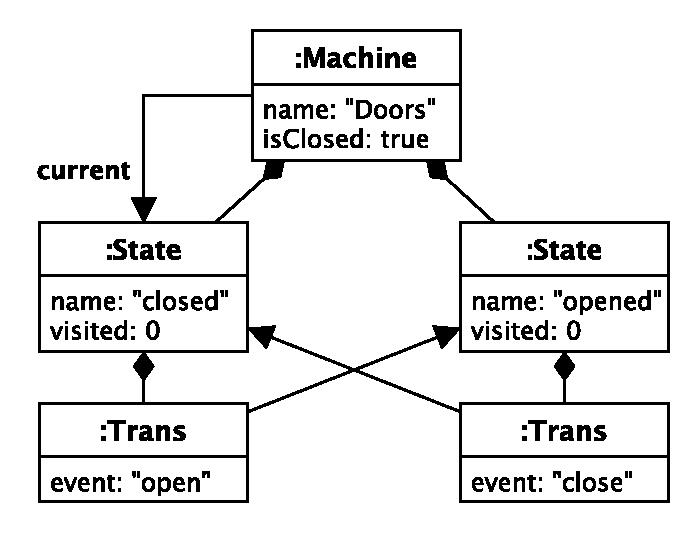
\includegraphics[width=0.5\textwidth]{figures/doorsmachine.pdf}
\caption{UML object diagram of the run-time structures of the Doors statemachine (excluding code objects)}
\label{FIG:doorsRuntime}
\end{figure}


An instance of a running state machine consists of an object graph conforming to the run-time schema of state machines, updating the \lstinline{current} state pointer in response to events. This object graph is graphically depicted in Figure~\ref{FIG:doorsRuntime} as a UML object diagram, excluding the statement objects representing on-entry actions. As the diagram shows, the running machine has a current state (\lstinline{closed}) and the \lstinline{isClosed} field has an actual value (\lstinline{true}). It is instructive to note that the diagram encode both static and dynamic aspects of the state machine language. Live editing the state machine then requires to \textit{patch}~\cite{SemanticDeltas} this run-time structure without shutting it down, possibly requiring migration of run-time state.

\subsection{Challenge}

\begin{table}[t]
  \centering
\begin{tabular}{lll}\toprule
\textsc{Change} & \textsc{What} & \textsc{How}\\\midrule
add & state & simple  \\
remove & state & structurally simple, but heuristic if state is current \\
rename & state & simple\\
add & variable & migrate class and initialize field \\
remove & variable & migrate class (NB: assumes variable is unused)\\
rename & variable & rename in class, preserving value\\
type change & variable & migrate class and convert or reinitialize value \\
add & transition & simple \\
remove & transition & structurally simple, but heuristic for pending events\\
event change & transition & structurally simple, but heuristic for pending events\\
add/remove & statement & hotswap code at quiescent point of interpreter\\
\bottomrule
\end{tabular}
\caption{Possible program changes and how to deal with them at run time}
\label{tbl:smchanges}
\end{table}

The space of possible (well-formed\footnote{The abstract syntax schema is not expressive enough to define all static invariants of the language, such as: states must by unique by name, references variables in actions must be declared, etc.}) changes to a state machine are summarized in Table~\ref{tbl:smchanges}.
The first column indicates the change category, the second the affected kind of object, and third a short description of how to deal with the respective change category. Some notes about this table:
\begin{itemize}
\item all rows with ``simple'' in the third column only require a quiescent~\cite{Tranquility} point in the interpreter loop to update the run-time structure (e.g., as shown in Figure~\ref{FIG:doorsRuntime}).
\item removing a state, however, is only \textit{structurally} simple, since removal is easy, but special care is required if the subject of removal is the current state. In this case, some heuristic is needed, such as: reject the edit, point the current state to the initial state, or some other strategy (e.g., the nearest state, previous state etc.)
\item everywhere a row mentions ``migrate class'' in the third column, data migration is needed: the run-time objects conforming to the old class must be transformed to instances of the updated class, similar to how Smalltalk migrates objects using \lstinline{become:}.
\item removing a transition or changing the event of a transition potentially has to deal with pending events (e.g., in an event queue) expecting such transitions, since such events are now potentially stale. Strategies to deal with this situation include: simply dropping the events, or requiring that such edits cannot be patched at run time when there are pending events.
\item the type change edit of variable requires a strategy for the current value: either discard and reinitialize, or perform value conversion. For instance, if the type change is from boolean to integer, then true could become 1, and false could become 0.
\item note finally that rename variable is mentioned explicitly as a change: this makes it possible to preserve the run-time value of the variable.
\end{itemize}

\subsection{Goals}

The goals for this challenge are twofold: from the end-user perspective and from the language engineering perspective. A particular challenge from the end-user perspective is to ``do minimal harm'': it is essential for fluid programming experience that the automatically triggered migrations are in a sense as near as possible to the previous application state, to not surprise or confuse the user/developer.
One approach  considered in earlier work~\cite{RuntimeConstraint} employs the constraint solver Z3 to find a ``nearest'' run-time instance compatible with a source change. Nevertheless, the patching of the run-time state should be quick enough so as to not disrupt the programmer experience.

From the language engineering perspective the goal is to employ techniques, formalisms, and tools, to make the construction of such languages easier. The above example state machine DSL is derived from earlier work~\cite{vanRozen19}, where the authors manually implemented the run-time patch operation and concluded that even for such a simple language (simpler even than the example above) it is a complex and error-pone endeavor. Furthermore, the field of software language engineering studies and develops generic and reusable techniques to improve the development of DSLs and programming languages, for instance, in the context of language workbenches~\cite{ERDWEG201524}. The development of live programming languages, however, is currently still out of reach for all existing language workbenches. The aforementioned approach using a constraint solver is an example of such a \textit{language parametric} technique, in that it operates on the (extended) abstract syntax metamodel of a language, and does not assume anything further about the language itself. Another approach is the \textsc{Cascade} metamodeling formalism which has builtin support for run-time patching~\cite{Cascade}. However, further research is needed to design better principled language engineering approaches that solve the problem in a way that is both declarative and fast.

\subsection{Extensions}

While the above example is arguably simple, the problem becomes much more challenging when the programs themselves define data types, classes, records, structures etc. Since possibly many instances (values, objects) of such data types may exist at run-time, these all have to be migrated in such a way that programmer experience is minimally disrupted, and that the invariants of said data types is maintained.
Another extension, tying in with the data-oriented examples above, involves refactorings of data types in a program. Typically a refactoring should be behavior preserving, but can it also preserve run-time data? The minimal example is the consistent variable rename rename in Table~\ref{tbl:smchanges}, which should not have any effect on run-time state.  A more complex refactoring is described in Section~\ref{sec:elm}.




\section{Related Work}
\label{sec:related}

There has been a lot of research on coordinating the evolution of interdependent layers of software, much of it guided by schema and types. But the vast majority of these techniques involve writing custom code in some specialized language, rather than through immediate action in an interactive programming system. Nevertheless it is important to understand these batch techniques to envision more interactive ones.

\paragraph{Schema evolution.}
Schema evolution has long been a major problem for SQL databases because
the SQL Data Definition Language (DDL) has limited capabilties to redefine existing data. It can rename tables and columns. SQLite \cite{sqliteDatatypes} uses dynamically typed values allowing them to be implicitly converted if the datatype of the column changes.
MYSql \cite{mysqlAlterTable} can reorder columns without destroying their data. But apart from such special cases, SQL databases have no general purpose support for data migration. As a result in practice schema evolution is mostly done by writing custom Data Manipulation Language (DML) code to migrate the data. Such custom code is greatly complicated if it needs to be done without taking the database offline or must be coordinated across multiple shards.
In \emph{Refactoring Databases} \citet{ambler06} offer a comprehensive taxonomy of schema evolution patterns, including typical strategies for online migration and sample SQL implementations.

\citet{bernstein07} observed in 2007 ``There are hardly any schema evolution tools today. This is rather surprising since there is a huge literature on schema evolution spanning more than two decades.'' There are now more tools available. Some tools such as Liquibase~\cite{liquibase} and PlanetScale\cite{planetscale} could be characterized as version control and continuous integration/deployment for schema. They track schema changes and can calculate diffs in the form of SQL DDL statements to convert one schema version to another, but do not help migrate data. Unfortunately comparing schemas can be ambiguous about the intention of changes. For example has a column been renamed or has it been deleted and a new one created? That distinction makes a big difference to the data in that column. EvolveDB\cite{evolvedb} addresses this ambiguity by reverse-engineering the schema into a richer data model and tracking the edits to that model within an IDE. This more precise edit history can be used to infer higher level intentions of a schema change, which then generate SQL scripts to evolve the database. EdgeDB~\cite{edgedb} resolves ambiguities by asking questions of the developer, with some answers supplying custom migration code in a proprietary query language.

Some tools provide a Domain Specific Language (DSL) to describe schema evolution. Rails Migrations~\cite{RailsMigrations} embeds a DSL in Ruby to manage schema migration but is comparable to the capabilities of SQL DDL, often requiring the addition of custom Ruby or SQL code. \citet{curino08} spawned a stream of research on Database Evolution Languages (DEL) by defining a Schema Modification Operator (SMO) as ``a function that receives as input a relational schema and the underlying database, and produces as output a (modified) version of the input schema and a migrated version of the database''. SMOs can also rewrite queries to accomodate schema changes. \citet{herrmann15} defined a relationally complete DEL and then extended it into a Bidirectional Database Evolution Language (BiDEL)~\cite{herrmann17}. BiDEL appears capable of handling the basic requirements of our \emph{Extract/Absorb Entity} and \emph{Multiplicity Change} challenges, though \emph{Split/Merge Entity} is less clear. It provides schema divergence by supporting multiple schema within one database, but would need some extension to handle data divergence.

\citet{wang19} use program synthesis to rewrite SQL programs to adapt to a schema change. This process is driven by finding possible correspondences between columns in the old and new schema guided by heuristics on textual similarity and confirmed by the existence of a synthesized equivalent program.
\begin{comment}
  I hate this paper - incredibly sophisticated techniques applied to an over-idealized problem. It is assumed the migration does not change datatypes or lose any information visible to the programs. It assumes the database has full code coverage. It ignores without explanation ambiguous schema changes (for example renaming equityped columns).
\end{comment}

Schema evolution is also a problem for NoSQL~\cite{sadalage12} databases. While such databases are sometimes called ``schemaless'' in effect that means the schema is left implicit and tools must try to infer it~\cite{storl20, storl22}. \citet{Cambria} uses lenses~\cite{Foster2007} for bidirectional transformation of JSON. \citet{scherzinger13} define a set of operators like the relational SMOs discussed above. \citeauthor*{chillon21}~\cite{chillon21, chillon22} offer a more comprehensive set of SMOs that may be capable of handling \textit{Extract/Absorb Entity} and \emph{Multiplicity Change} but not \emph{Split/Merge Entity} nor divergence. None of the above approaches to NoSQL evolution have yet extended into updating code or rewriting queries like their SQL cousins.

\emph{Local-first software}~\cite{localfirst} adds the divergence dimension to NoSQL evolution, because the code running on different replicas can evolve at different paces. \citet{Cambria} applies lenses~\cite{Foster2007} to this problem, specifically discussing the \emph{Multiplicity Change} problem.

Schema evolution has also been studied for Object Oriented Databases(OODB)~\cite{li99,banerjee87}. Smalltalk~\cite{Goldberg80} is itself an OODB, persisting all object instances in an ``image file'' with some evolution capabilities incorporated in the programming environment~\cite[pp.252-272]{Goldberg80}. Gemstone turns the Smalltalk image into a production-quality database and accordingly provides a complex schema evolution API~\cite{Gemstone}.

\paragraph{Type-driven transformations.}
Programming language theory undergirds research on type-driven transformations. Bidirectional Transformations~\cite{czarnecki2009bidirectional} have been used for data format conversion and view update.
Coupled Transformations~\cite{Berdaguer07, alcino06, Cleve2006} express transformations coordinated between types and their instances by encoding them into functions on Haskell GADTs built with strategy combinators. \citet{JVisser08} extends the encoding to transform queries written in point-free style. \citet{lammel16} recapitulates coupled transformations within logic programming which extends it to transform logic programs. It is not clear how bidirectional transformations can handle generating the unique IDs required in some evolutions, nor the information loss and duplication which can arise in some divergence scenarios.

\paragraph{Model Driven Engineering.}
Model Driven Engineering must also handle evolution. Unlike the textual artifacts involved in other domains, models typically assign unique indentifiers enabling more precise differencing and mergeing~\cite{alanen2003}.
Models are often themselves modeled by a metamodel, which lifts the evolution problem to the metalevel: models must be migrated through the evolution of their metamodel, analogously to changing the grammar of a programming language.~\cite{Herrmannsdoerfer11}. \citet{Cicchetti11} study metamodel evolution in the context of divergent changes.
\citet{vermolen11} define a DSL for evolving a data model by generating SQL migrations on the backing database. They consider the evolution of OO-style subclass hierarchies which goes beyond most other work. Their running example includes both our \emph{Extract Entity} and \emph{Multiplicty Change} examples, and would make for a good follow-on problem. However they do not address code/query rewriting.

\paragraph{Migration by example.}
Programming by example has been used to infer schema migration programs from examples specified by the developer~\cite{wang20, Alexe11}.
This work deals with the reality that schema live in the database and so examples must be supplied separately, but we wonder why not incorporate examples into a schema definition language? Textual edits to schema in this language would also adapt the examples, which then could be used to infer an abstract migration, thus avoiding the ambiguities of textually comparing pure schema.

\paragraph{Data wrangling.} The evolution of data formats is a concern in Data Science. Data~Diff~\cite{sutton18} compares two versions of tabular data and finds a minimal matching transformation.
Wrangler~\cite{kandel11} observes interactive manipulation of sampled data to write data transformation programs.
\citet{petersohn20} present an algebra of operations on Python dataframes that include shape transformations.

\paragraph{Live programming.}
Live programming~\cite{tanimoto90, rein2018exploratory} seeks to speed up feedback in (primarily solo) programming.
% \cite{mcdirmid13, Rauch_2019, beckmann2021shortening}
\emph{Hot reloading/swapping}~\cite{barenz2020essence, hicks2005dynamic} installs code changes into a running system preserving some runtime state but not attempting to migrate that state through type changes.
\citet{SemanticDeltas} proposes a research agenda for thoroughly live DSL programming focusing on \emph{Semantic Deltas} that unify edit-time and run-time change.
\citet{RuntimeConstraint} study the live modeling problem in Section \ref{livemodeling}. They use constraints supplied by the developer to solve for the best new runtime state following a DSL language evolution. \citet{vanRozen19} take an alternative approach to the same problem using \emph{origin tracking} in textual editing.
%\citet{vanRozen23} subsequently proposed a metaprogramming language for live DSL programming.


%\paragraph{collaborative programming tools}\cite{goldman2011real,kurniawan2015coder,replit}


%\bibliographystyle{abbrv}
%\bibliography{paper}
\printbibliography


\appendix

\section{\textcolor{red}{[TVDS] Super rough attempt at the paragraph}}

Modern day software development is collaborative. Single user programming does not exist anymore.
Just as document editing is becoming more collaborative through online systems like pioneered by Google Docs,
programming would benefit form online collaboration. In a sense this is live programming++: whereas traditional
live programming systems assume a single developer editing code and see their changes immediately reflected
in the running system, online collaborative programming is the same but for multiple programmers at the same time.
The key challenge here, we posit, the *schema change*. We take inspiration from database migration,
model evolution, and version control, and identify benchmark problems. This is already evident in live programming:
editing a program, consisting of type definitions defining the structure run-time state and (transient) procedures, functions
etc. operating on that state, requires run-time state to be migrated, after the programmer edits their program.
Adding the dimension of multiple programs brings us into the domain local-first, and decentralized version control, where
copies are created and edited, which eventually have to be reconciled again (e.g., through merging).
Whereas schema evolution and its associated migration problems has seen a lot of attention in the database world,
the model-driven world, and the bidirectional transformation (BX) communities, the techniques are still too low-level,
too manual, and too much focused on a single user perspectives. By identifying the similarities between analogous
problems in live, multi-user programming systems, we hope to stimulate further research on more comprehensive, automatic,
high-level, and online solutions. So that the benefits of live programming can be enjoyed in a global and distributed setting
involving multiple programmers at the same time.

\section{\textcolor{red}{[JE] Type evolution for live programming}}

Many past improvements in the practice of programming worked by speeding up feedback loops. Live Programming aspires to the optimum of immediate feedback. The problem is that modern software is built out of many layers of different technologies -- thoroughly live programming would propagate changes immediately up and down the entire stack of a running system, from the database to the code, and from the client to the server. We call this \textit{full-stack} live programming. Another problem is that modern software is built with complex collaborations involving development, testing, deployment, and suppport. Such workflows are themselves feedback loops -- thoroughly live programming would propagate changes between participants frictionlessly. We call this \textit{end-to-end} live programming.

We propose a research agenda towards this greater vision of live programming. The starting point is database \textit{schema evolution}, which propagates database schema changes into data migrations and query rewriting. We call for generalized \textit{type evolution} that works immediately across the entire software stack, and automatically across the entire software workflow. This paper contributes a set of challenge problems to serve as targets for research on type evolution and as a basis of comparison for the results.

\section{\textcolor{red}{[GL] Rough paragraph}}

Most programming languages analysis treats state as ephemeral: tied to the lifetime of a running program, and reset when the program is edited. But when we take a broader view, most \textit{programming systems} (cite) have state that lasts beyond the lifetime of a single execution. This includes collaboration applications with state persisted in a database, image-based systems like Smalltalk, and live programming environments where the program can be edited without resetting all state.

Although these programming systems exist in very different contexts, they all encounter similar problems related to the essential difficulty of preserving state across program edits. New versions of the program must correctly handle pre-existing data. When the data schema or type definitions change, existing data must be evolved to conform to the new schema. Changing data representations or types can also require changing corresponding parts of the program. These problems have been noticed, named, and studied in these different programming systems: ``schema evolution'' in the databases literature, ``hot reloading'' in live programming, etc.

In this paper, we draw connections between these different contexts, pointing out essential shared structure in the hopes of motivating further research on this important problem and encouraging knowledge sharing across subfields. Our contributions are: 1) a shared framework for thinking about the relationship between schema, code, and data in a programming system, 2) Case studies of the framework in a highly diverse set of programming systems, motivated by real-world examples.


\section{\textcolor{red}{[TP] Rough paragraph}}

Programming is increasingly collaborative and interactive. We welcome this trend, because
greater collaboration and interactivity make programming more effective. Future programming
environments enable programmers to collaborate at a more fine-grained level, adopting individual
code changes created by their collaborators as needed. They also let programmers interactively
edit code, often during program execution.

In order to support this new way of working, programming systems increasingly have to tackle the
problem of schema evolution. If a programmer imports a change that edits a schema, code and data
that relies on such schema needs to be adapted to match the new schema. Similarly, if a programmer
in a live programming environment modifies their type definition, current program state needs to
be updated to match the new structure of types. This is a well-understood and well-studied problem
in database community, but it has received little attention in work on programming systems.

The aim of this paper is to provide a conceptual framework for talking about schema evolution in
collaborative and live programming systems. Taking inspiration from Stewart Brand's analysis of
pace layers, we propose to think of the problem as the problem of evolution of occuring at three
layers, the most permanent schema layer, less permanent code layer and least permanent data layer.
A change at the most permanent layer affects the less permanent layer, which then has to be
updated to keep correspondence between the layers.

We consider four case studies of such schema evolution in collaborative and live programming
systems. We present those throught the perspective of our unified conceptual framework. The work
both sheds a new light at how schema change needs to be handled in programming systems and also
provides a range of challenges that show interesting problems that future programming systems
will need to tackle.


\section{Introduction}

\textcolor{red}{[JE] We should adopt the term Schema Evolution, which is favored in the research literature, defined to include schema change, data migration, and query rewriting. }

Schema change won't go away. Changing requirements and changing code lead to changing the schema of a database. Schema change, also called schema migration, is the problem of migrating existing data from the old schema to the new. This often involves custom migration programs or specialized Domain Specific Langiuages. The migration must be carefully coordinated with upgrading the application code and associated artifacts that assume the new schema. Schema change on database servers is often delegated to Database Administrators and DevOps. Live programming~\cite{tanimoto90,Hancock03} and local-first software~\cite{localfirst} both move data away from the server, eliminating those jobs, but not eliminating the need to do schema change, and indeed increasing the need to do it automatically. Recently \citet{Cambria} spotlighted these problems and proposed an approach using lenses~\cite{Foster2007}, but otherwise there has been surprisingly little research. To promote further progress we offer a set of challenge problems to the live programming and local-first communities, inviting them to propose and compare solutions.

Live programming seeks to erase the boundary between editing and running programs. In order to do so program data must be kept around while the program is being edited. Classic Lisp and Smalltalk systems integrated code and data into a persistent \textit{image}~\cite{Sandewall78, Goldberg80}. An interactive shell or \textit{Read Eval Print Loop (REPL)}~\cite{Deutsch64} is more transient than an image, but still builds up a context of data over long-lived programming sessions the loss of which disrupts the programmer's workflow. In all of these environments programs eventually get changed to create and expect data in a form incompatible with extant data. This happens whether or not the form of the data is specified explicitly in a type system or database schema, or whether it is left implicit in the behavior of the code. Some languages can tolerate a larger set of such changes, most notably Smalltalk which will automatically insert and delete members in existing instances when a class definition is changed~\cite[pp.252-272]{Goldberg80}.\footnote{Gemstone turns the Smalltalk image into a production-quality database and accordingly provides a sophisticated schema change API~\cite{Gemstone}. Schema change won't go away.} But there is still a large class of changes that create incompatibilities with existing data, whether it is inside an image, programming environment, REPL, or an external database. Some live programming environments generate data with unit tests, but that only shifts the problem of schema change to adapting those tests. One way or another, stopping everything to manually deal with schema change contradicts the goals of live programming. Schema change won't go away.

Local-first software faces related problems. Its goal is to empower users by moving code and data from the cloud to the user's own devices. Distributed programming techniques like Convergent Replicated Data Types (CRDTs)~\cite{Shapiro11} are used to coordinate data changes peer-to-peer. Unfortunately these techniques so far have not addressed schema change nor code deployment The traditional techniques of schema change used in centrally managed databases are complicated by the distributed and intermittently connected nature of local-first data. Schema change won't go away.

In the following sections we present a series of challenge problems dealing with schema change in the context of live programming and local-first software. These problems are necessarily expressed using established idioms or conventions, but nevertheless we welcome solutions that translate the spirit of the problem into other contexts.

~

~

\textcolor{red}{TODO: Need to explain that we take the programming system view - program is not something
built centrally, but something that exists and can be modified}

~

\textcolor{red}{TODO: Maybe the right way to frame this is to say that the challenges are intended
less for evaluating particular solutions but more for framing and making sense of different
kinds of schema-change-related problems.  You can read this paper and when you face a schema-change-related
problem, think about it in terms of our dimensions. Maybe compare it to our challenges.
We do not necessarilly expect that people will directly solve our challenges though. (Although
some might and that would be nice..)}

~

\textcolor{red}{TODO: I also guess this is more about just ``change'' than ``schema change''
which is one particular (most challenging) instance - i.e., change at the most permanent
pace layer.}

\end{document}

% Local Variables:
% TeX-engine: luatex
% End:
